\documentclass[parskip=full]{scrartcl}
\usepackage[utf8]{inputenc} % use utf8 file encoding for TeX sources
\usepackage[T1]{fontenc}    % avoid garbled Unicode text in pdf
\usepackage[german]{babel}  % german hyphenation, quotes, etc
\usepackage{hyperref}       % detailed hyperlink/pdf configuration
\hypersetup{                % ‘texdoc hyperref‘ for options
	pdftitle={Bericht},%
	bookmarks=true,%
}
\usepackage{graphicx}       % provides commands for including figures
\usepackage{csquotes}       % provides \enquote{} macro for "quotes"
\usepackage{scrpage2}
\usepackage{caption}
\usepackage{enumitem}
\pagestyle{scrheadings}
\usepackage{float}

%\clearscrheadfoot
\ohead{BPTI: Gruppe 03=\{Niklas Metz, Felix Bachmann\}, Bericht, WS 2017/18}

\title{BPTI: Bomberman in VHDL}
\subtitle{von Niklas Metz und Felix Bachmann}

\begin{document}
	\maketitle
	\newpage
	\tableofcontents
	\newpage
	
	\part{Allgemeines}
		\section{Idee}
			Die grundlegende Idee war ein klassisches Bomberman-Spiel, wie man es von älteren Konsolen kennt. Zwei Spieler können sich auf einem Spielfeld bewegen und Bomben platzieren, um Blöcke oder den Gegner zu zerstören.
			\begin{figure}[H]
				\centering
				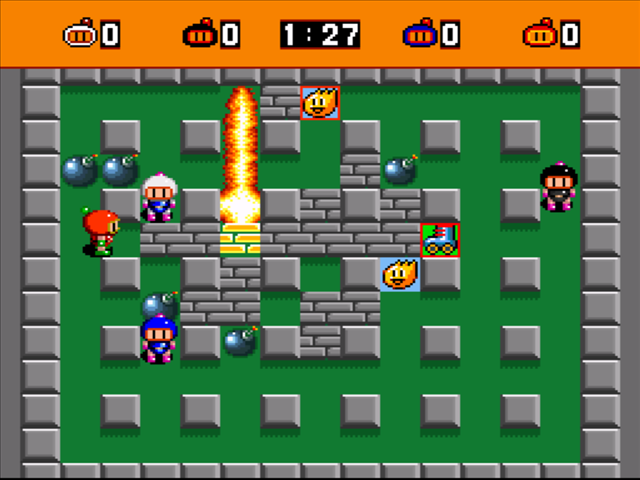
\includegraphics[scale=0.4]{./bilder/bomberman.png}
				\caption{Screenshot eines Bomberman-Spiels}
			\end{figure}
		
		\section{Erreichte Ziele}
			%TODO bildschirmfoto
			Wir haben alle unsere Musskriterien erfüllt. Es gibt zwei Spielfiguren, die sich von den Spielern steuern lassen und sich nicht über Blöcke bewegen können. Das Spielfeld ist durch unzerstörbare und  zerstörbare Blöcke sowie leere Felder aufgebaut. Jeder Spieler kann eine Bombe platzieren, die nach einer bestimmten Zeit explodiert. Bei der Explosion werden zerstörbare Blöcke, die sich im Radius der Explosion befinden zerstört. Ebenfalls sterben Spieler, die sich in einer Explosion befinden. \newline
			Außerdem haben wir Sprites für alle Blöcke und auch für die beiden Spieler implementiert. \newline
			
		
		\section{Steuerung}
			%TODO Bild vom Controller
			%TODO Bild von der Verkabelung?!?!
			\begin{table}[H]
				\centering
				\label{controls}
				\begin{tabular}{|l|l|}
					\hline
					\textbf{Knopf} & \textbf{Wirkung}      \\ \hline
					1           & Hoch \& Runter bewegen               \\ \hline
					2           & Bombe platzieren                 \\ \hline
					3           & Links \& Rechts bewegen                    \\ \hline
				\end{tabular}
				\caption{Steuerung}
			\end{table}
			
	
	\part{Beschreibung der Entities}
		\section{bomberman\_ent}
			%TODO blockdiagramm
			bomberman\_ent ist die Top-Level-Architektur. Die Eingänge sind die tatsächlichen Eingaben des Nutzers und auf den Ausgängen liegen die Informationen die für den VGA-Anschluss benötigt werden. in bomberman\_ent werden drei Entities miteinander verbunden. Zuerst die sync\_gen\_ent, die hsync und vsync erzeugt. Außerdem die game\_mechanic\_ent, welche die eigentliche Spiellogik enthält. Zuletzt noch die graphics\_ent, die für die Erzeugung der entsprechenden RGB-Farbwerte zuständig ist. 
			Letzere enthält ausschließlich asynchrone Entities, sync\_gen\_ent und game\_mechanic\_ent enthalten ausschließlich synchrone Entities (wenn nicht anders angegeben, kriegen diese die VGA-Clock als Takt).
			In bomberman\_ent werden außerdem die beiden Generics TILE\_SIZE und PLAYER\_SIZE definiert und mit 32 initialisiert.
		
		\section{game\_mechanic\_ent}
			%TODO blockdiagramm
			game\_mechanic\_ent ist die Architektur, welche die eigentliche Spiellogik enthält. Hier werden zwei Spieler vom Typ player\_ent erzeugt und mit der Logik in game\_state\_ent verbunden. Außerdem wird hier entschieden welche Zeilen an die einzelnen Spieler weitergegeben werden. Jeder Spieler benötigt lediglich die Zeile in der er sich befindet, sowie die über und unter ihm, um zu entscheiden, ob er sich in eine bestimmte Richtung bewegen kann. 
		
			\subsection{game\_state\_ent}
				game\_state\_ent ist einerseits für die Verwaltung des Speilfeldes, aber auch für die Kollisionen verantwortlich. Unser Spielfeld besteht aus insgesamt 15 Zeilen mit jeweils 15 Spalten, wobei jedes Feld durch vier Bits kodiert wird. Die genauen Kodierungen der einzelnen Blöcke kann man Tabelle 1 entnehmen. In dieser Entity wird der Anfangswert für alle Zeilen des Spielfeldes bestimmt, die durch das Ablaufen des Spiels verändert werden können. \newline
				Sollte ein Spieler seine Bombe legen, bekommt game\_state\_ent die Postion der Bombe, sowie die Information, dass die Bombe gelegt wurde. Daraufhin wird die entsprechende Zeile so geändert, dass die Bombe auch tatsächlich sichtbar ist. Nachdem der Zähler der Bombe abgelaufen ist und sie explodieren soll, wird das entsprechende explode Signal gesetzt. Dann werden die umgrenzenden Blöcke der Bombe überprüft und auf Explosionen gesetzt. Die Blöcke müssen zuerst überprüft werden, um zu verhindern, dass unzerstörbare Blöcke von den Explosionen zerstört werden. Wenn der entsprechende Explosions Zähler in der Bombe abläuft, wird das explosion Signal auf 0 gesetzt und die Felder mit Explosionen werden auf leere Felder geändert. \newline
				Desweiteren werden hier die Kollisionen der Spieler erkannt. Sollte sich ein Spieler auf einem Feld befinden, auf dem momentan eine Explosion ist, wird das enable Signal des Spielers auf 0 gesetzt und er "stirbt". Dabei verwenden wir jeweils den Mittelpunkt des Spielers als Vergleichswert, um zu entscheiden ob er stirbt oder nicht. \newline
				
				\begin{table}[H]
					\centering
					\label{tileCode}
					\begin{tabular}{|l|l|}
						\hline
						\textbf{TileID} & \textbf{Bezeichnung}      \\ \hline
						0x0           & Leeres Feld               \\ \hline
						0x1           & Explosion                 \\ \hline
						0xD           & Bombe                     \\ \hline
						0xE           & Zerstörbarer Block        \\ \hline
						0xF           & Unzerstörbarer Block      \\ \hline
					\end{tabular}
					\caption{Spielfeld-Kodierungen}
				\end{table}

			\subsection{player\_ent}
				Die Entity player\_ent enthält alle Unterkomponenten eines Spielers. 
				Diese sind eine bomb\_ent und movement\_ent (inklusive Clock), da jeder Spieler eine Bombe legen kann und bei Bewegungen auf Kollision mit Kacheln überprüft werden muss.
				Als Eingabe erhält player\_ent die VGA Clock, ein asynchrones Reset, sowie alle Eingaben des Gamepads (Bewegung in alle 4 Richtungen und den Knopf zum Bombe legen) und einen enable-Eingang. Letzterer verhindert, dass ein Spieler, der bereits von einer Bombe getötet wurde, noch Bomben legen kann. Weitere Inputs sind die Rows des Spielfeldes, welche sich um die aktuelle Spielerposition herum befinden.
				Als Ausgabe hat player\_ent die aktuelle Position des Spielers (pixel- als auch kachelweise). Außerdem wird die Kachel-Position und der Zustand der Bombe ausgegeben.
				
				\begin{figure}[H]
					\centering
					%TODO\includegraphics[scale=0.4]{}
					\caption{Blockdiagramm player\_ent}
				\end{figure}
				
				Bemerkung zur Abbildung: Neben der normalen Verdrahtung wenden wir in player\_ent noch eine Transformation von Pixel- auf Kachelkoordinaten an. Der Übersichtlichkeit halber haben wir dies nicht als asynchrone Entity modelliert, sondern direkt in die strukturelle Beschreibung eingefügt (beim Abbilden der forward-Signale auf die Out-Ports).
				\subsubsection{clk\_movement\_ent}
				Die Entity clk\_movement\_ent ist ein Clock Divider, die Architecture wird funktional beschrieben. Die Entity wird genutzt, um die Geschwindigkeit der Bewegung der Spieler zu steuern. Es wird alle 78125 Originaltakte die Ausgabe Ausgabe negiert. Da in unserem Design die VGA-Clock genutzt wird, wird somit alle $\frac{78125 * 2}{25.175 * 10^6}s \approx 6.2ms$ ein Takt erzeugt. Dies hat zur Folge, dass bei ständiger Bewegung eines Spielers in die gleiche Richtung, die pro steigender Takt-Flanke des ausgegebenen Takts stattfindet, die Bewegung vom linken bis zum rechten Rand des Spielfelds (480 Pixel) $480 * 6.2 ms \approx 2.98 s$ dauert. Diesen Wert haben wir bei BombermanGB über einen Emulator gemessen und \enquote{rückwärts} den nötigen Zähler, also 78125, bestimmt.
				\subsubsection{movement\_ent}
					Die Entity movement\_ent wird durch eine Architecture funktional beschrieben und ist für die Bewegung eines Spielers zuständig. Als Eingangssignale erhält die Entity die von clk\_movement\_ent generierte Clock. Weitere in-Ports sind die low-aktiven Signale des Gamepads zum Bewegen des Spielers. Zuletzt kennt die Entity durch Eingangssignale auch den Zustand des Spielfeldes. Dieser wird benötigt, um die Kollision des Spielers mit Blöcken zu prüfen.
					Die Ausgabe ist die Pixel-Position des Spielers.
					Diese wird anhand der gewünschten Bewegungsrichtung (durch die Gamepad-Signale gegeben), der in der Entity gespeicherten Pixel-Position vor der Bewegung und des aktuellen Zustandes des Spielfelds berechnet. Die Pixel-Position wird um eine in der Entity definierte Konstante verändert, falls keine Kollision mit einem Block auftritt. Jede Kachel, die nicht leer ist, führt dabei zu einer Kollision.
					Der Test auf Kollision wird jedoch nur durchgeführt, falls durch die Bewegung eine Kante des Spielers auf eine Kachel bewegt werden würde, auf der sich der Spieler vorher nicht befand. \newline
					Beispiel: Sei die Spieler- und Kachelgröße 32x32 Pixel. Die Koordinaten beginnen bei (1,1). Dann wird bei einer Bewegung nach links nur auf Kollision überprüft, falls $((x-1)$ mod $32) == 0$. Nur in diesem Fall wird eine andere Kachel betreten.\newline
					Dadurch ist es dem Spieler möglich von einer Kachel, auf der er eine Bombe gelegt hat, zu entkommen (die Bombe würde auch zu einer Kollision führen).
					Die Bewegung in x- und y- Richtung kann , falls möglich, parallel geschehen.
				\subsubsection{bomb\_ent}
					Die Entity bomb\_ent enthält die funktionale Beschreibung einer Bombe. Als Eingabe erhält die Entity die Kachel-Position des zugehörigen Spielers, um beim Legen einer neuen Bombe die Position derselben festlegen zu können. Weitere in-Ports sind das low-aktive Signal des Knopfes auf dem Gamepad zum Legen einer Bombe und das enable-Signal des zugehörigen Spielers. Letzteres wird benötigt, um zu verhindern, dass ein bereits toter Spieler eine neue Bombe legen kann.
					Die Ausgabe sind die Kachel-Position der Bombe, sowie ein enable- und ein explode-Signal. Beide Signale zusammen ergeben die verschiedenen Zustände der Bombe.
					\begin{table}[H]
						\centering
						\label{bombCode}
						\begin{tabular}{|l|l|}
							\hline
							\textbf{enable, explode} & \textbf{Zustand}      \\ \hline
							0,0         & Bombe ist nicht aktiv              \\ \hline
							0,1           & ungültiger Zustand               \\ \hline
							1,0          & Bombe ist auf dem Spielfeld, explodiert aber noch nicht \\ \hline
							1,1          & Bombe ist auf dem Spielfeld und explodiert     \\ \hline
						\end{tabular}
						\caption{Zustände der Bombe}
					\end{table}
					Zur Generierung dieser Signale finden sich in der Architecture zwei Counter. Sobald erfolgreich eine neue Bombe gelegt wurde, wird das enable-Signal auf 1 gesetzt und ein Counter beginnt. Dieser zählt (falls die VGA-Clock als Takt genutzt wird) circa drei Sekunden und symbolisiert das \enquote{Ticken} der Bombe. Sobald dieser Counter heruntergezählt hat, wird das explode-Signal auf 1 gesetzt und der zweite Counter beginnt zu zählen. Dieser zählt circa eine halbe Sekunde. Hat dieser Counter heruntergezählt wird das explode-Signal und das enable-Signal auf 0 gesetzt. Der zweite Counter wird benötigt, damit die Explosion einer Bombe eine gewisse Zeit andauert und auf dem Bildschirm für das menschliche Auge sichtbar wird.
					\begin{figure}[H]
						\centering
						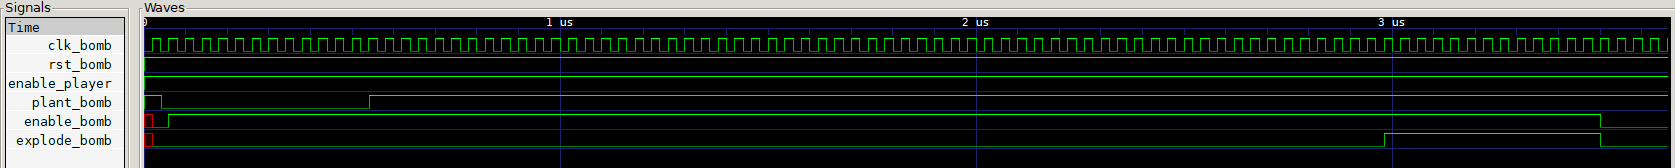
\includegraphics[scale=0.4]{./bilder/bomb_sim.png}
						\caption{Simulation von bomb\_ent \newline(Takt-Dauer von 40 ns, Counter um 6 Größenordnungen verringert)}
					\end{figure}
			
		\section{graphics\_ent}
			graphics\_ent kapselt die Farbenerzeugung. Als Eingabe bekommt es die Informationen über die Positionen der Spieler und über das Spielfeld, sowie die Position des aktuell zu zeichnenden Pixels (generiert durch sync\_gen\_ent). Aus diesen Werten, wird durch pixel\_gen\_ent entschieden welche Sprites gerade verwendet werden müssen. Anschließend werden die ausgelesenen Farbinformationen in rgb\_assign\_ent auf die einzelnen Farbausgänge gelegt.\newline
			
			\begin{table}[H]
				\centering
				\label{spriteCode}
				\begin{tabular}{|l|l|}
					\hline
					\textbf{SpriteID} & \textbf{Bezeichnung}      \\ \hline
					0x0           & Leeres Feld               \\ \hline
					0x1           & Explosion                 \\ \hline
					0x2           & Spieler 1                 \\ \hline
					0x3           & Spieler 2                 \\ \hline
					0x4           & Kodierung für schwarzen Rand \\ \hline
					0xD           & Bombe                     \\ \hline
					0xE           & Zerstörbarer Block        \\ \hline
					0xF           & Unzerstörbarer Block      \\ \hline
				\end{tabular}
				\caption{Sprite-Kodierungen}
			\end{table}
		
			\begin{figure}[H]
				\centering
				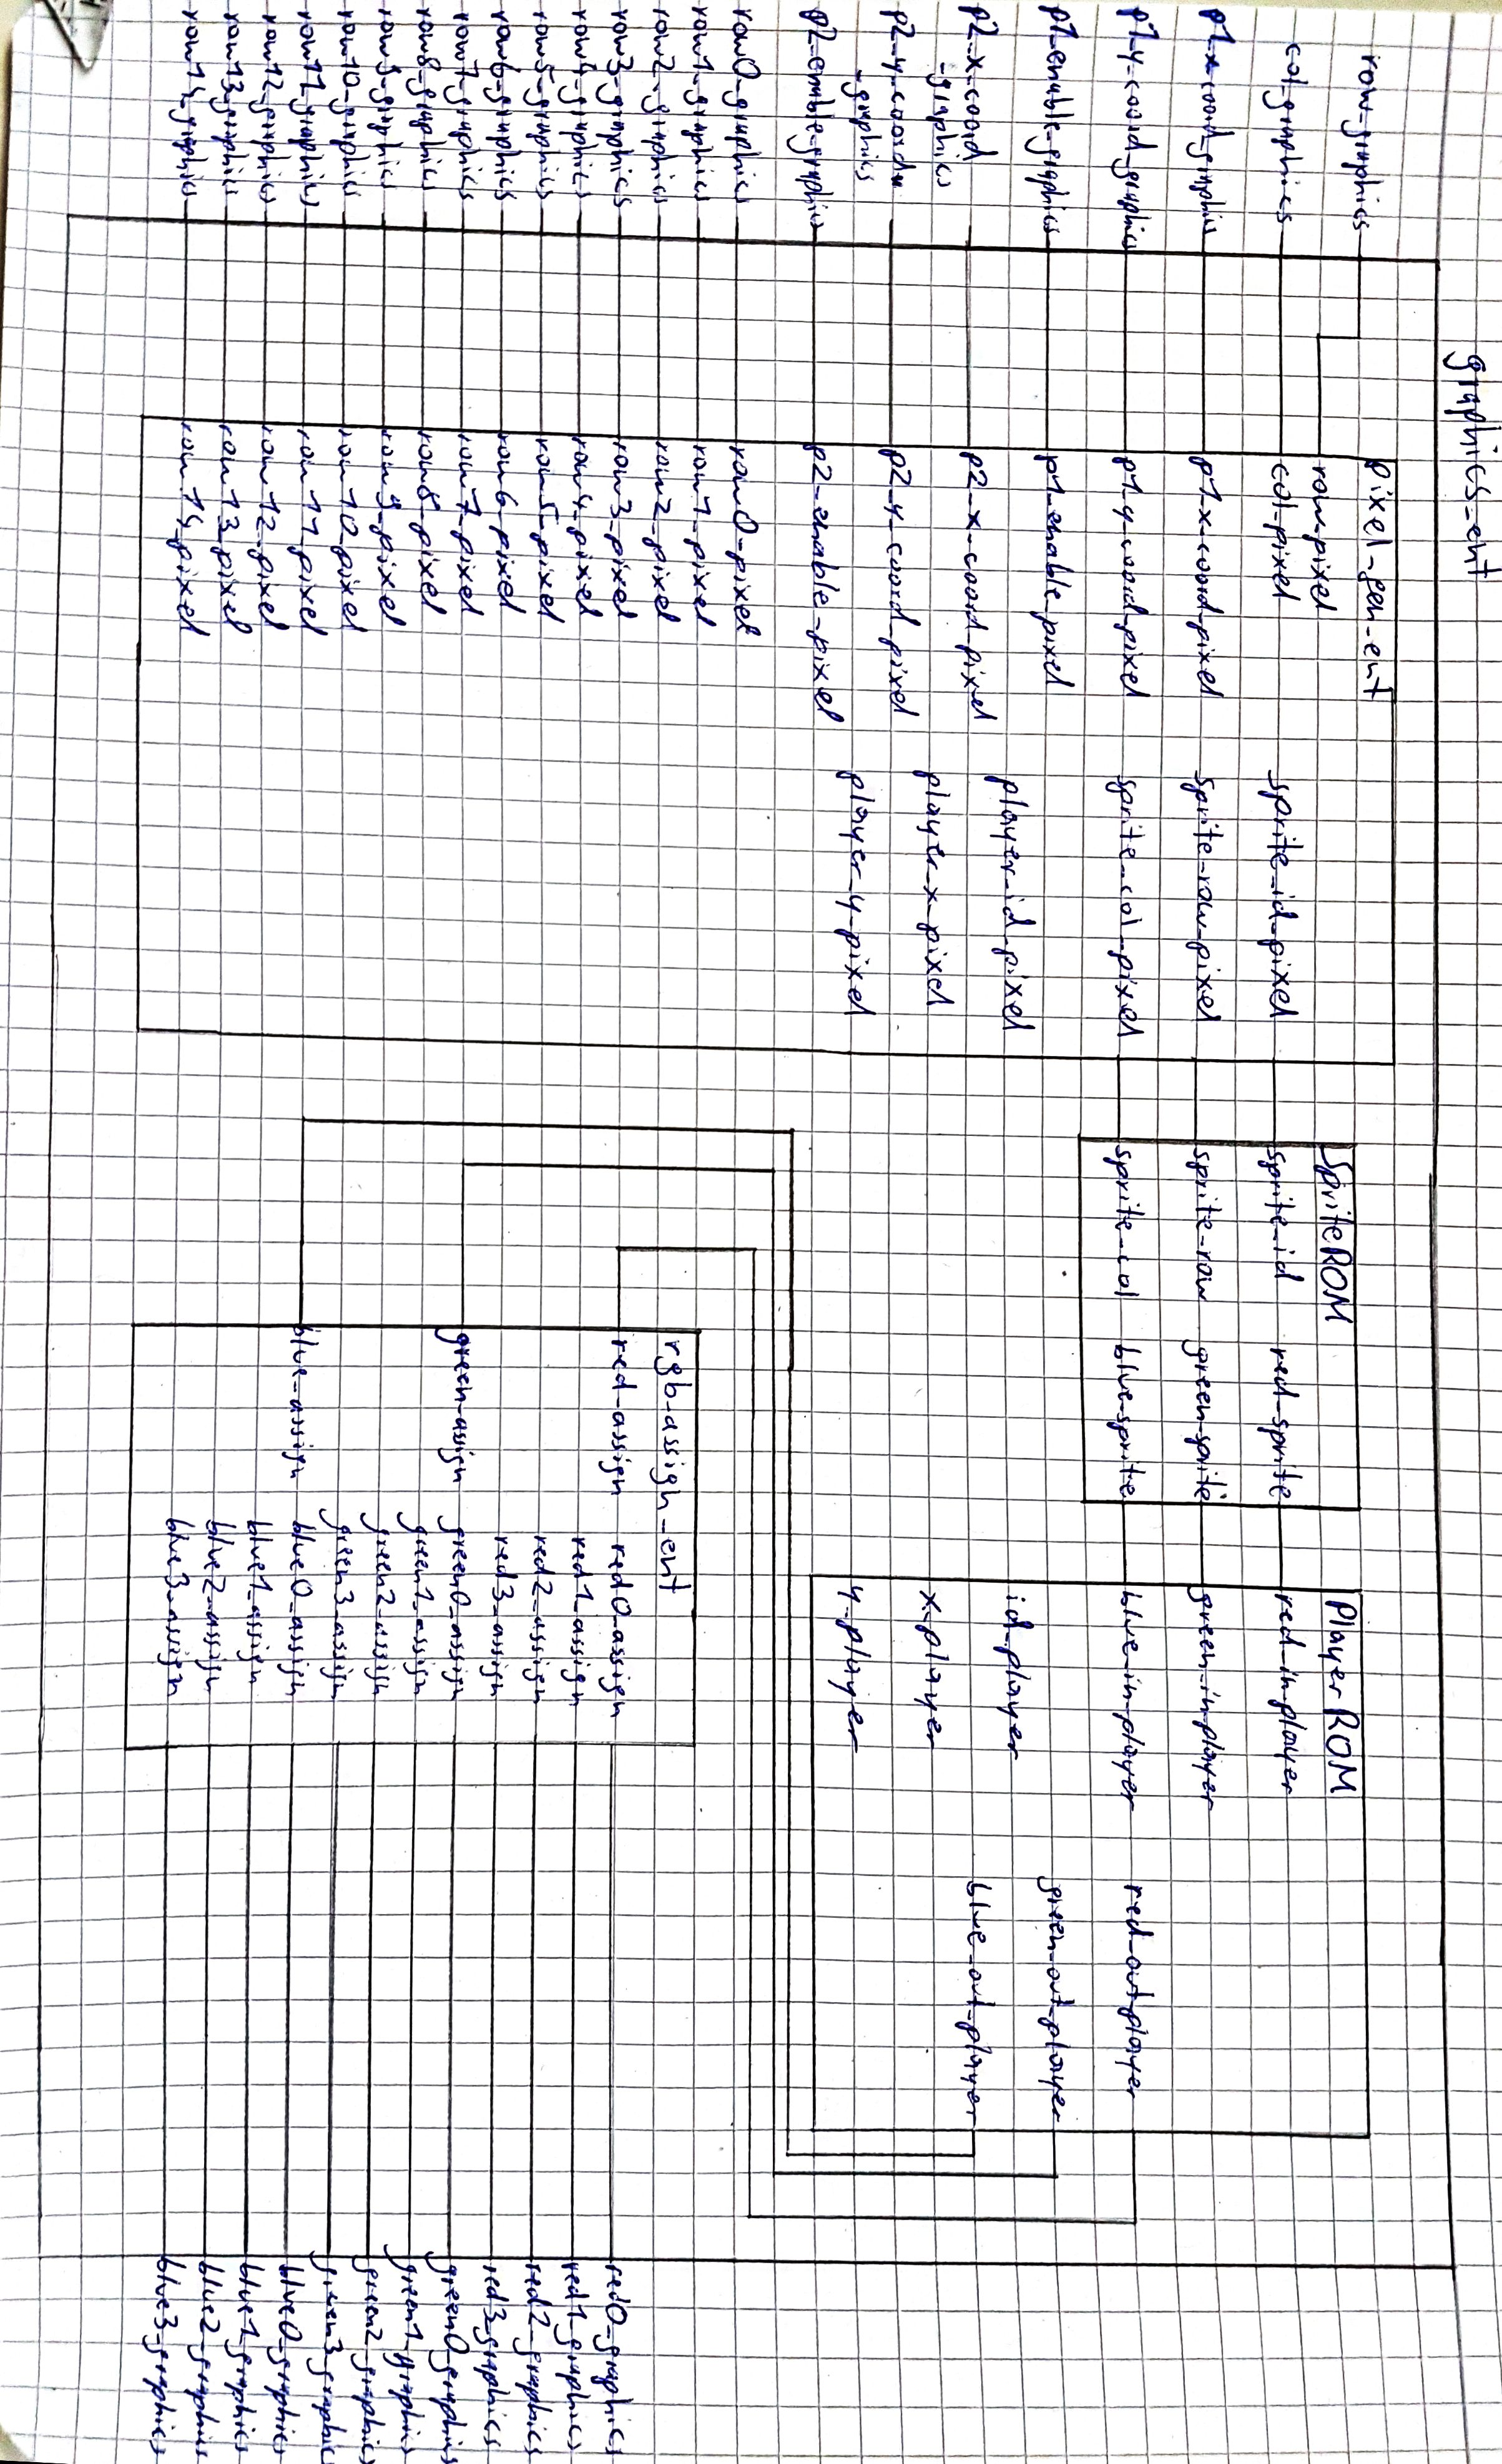
\includegraphics[angle=90,scale=0.1]{./bilder/graphics_ent.jpg}
				\caption{Blockdiagramm graphics\_ent}
			\end{figure}
			
			\subsection{pixel\_gen\_ent}
				pixel\_gen\_ent bekommt als Eingaben die Informationen über die Spieler, sowie über das Spielfeld. Abhängig von diesen Informationen gibt die Entity aus, auf welche Sprites zugegriffen werden soll und an welcher Stelle.\newline
				Die 160 Spalten am linken Rand des Monitors werden bei uns dauerhaft schwarz gefärbt, da wir ein quadratisches Spielfeld wollten, was allerdings bei einer Auflösung von 640x480 nicht funktioniert. Unser tatsächliches Spielfeld ist somit nun 480x480 Pixel groß.\newline
				Der erste Spieler hat bei uns den Vorrang vor dem zweiten Spieler, also falls sich beide Spieler übereinander befinden, wird der erste Spieler gezeichnet.\newline
				Wir haben unterschiedliche Ausgänge für die Informationen über die Sprites für Spielfeld und Player, um im PlayerROM entscheiden zu können ob wirklich der Spieler oder doch das Spielfeld gezeichnet wird, falls die Grafik des Spielers an der bestimmten Position transparent ist.
		
			\subsection{Sprites}
				In den beiden Entities PlayerROM und SpriteROM befinden sich Sprites, die in Abhängigkeit des aktuellen Zustands der Arena, der Spieler und der Bomben RGB-Werte an den VGA-Controller ausgeben. Dazu befinden sich in den beiden Entities PlayerROM und SpriteROM pro Sprite (es existieren Sprites für: Spieler 1, Spieler 2, leerer Block, zerstörbarer Block, unzerstörbarer Block, Bombe, Explosion) ein zweidimensionales konstantes Array (wird synthetisiert als ROM). Diese Arrays sind jeweils 32 * 384 Bit groß. \newline
				Die Größe ergibt sich folgendermaßen: Die Kacheln des Spielfeldes sowie die Quellsprites haben eine Größe von 32 * 32 Pixel. Da für jeden Farbkanal des VGA-Ausgangs 4 Bit zur Verfügung stehen haben wir in dem Array den RGB-Wert jedes Pixels mit 3 * 4 Bit (also 3 Hex-Werte) kodiert. So kommen 32 Zeilen mit jeweils 
				3 * 4 * 32 = 384 Bit zustande. \newline
				Die Sprites haben wir aus einem Sprite-Sheet von opengameart (\url{https://opengameart.org/sites/default/files/DungeonCrawl_ProjectUtumnoTileset.png}) ausgeschnitten und mithilfe eines Java-Programmes, welches im Abgabe-Verzeichnis zu finden ist und im folgenden kurz beschrieben wird, in VHDL-Arrays umgewandelt.
				\subsubsection{SpriteExtractor.java}
					Das Java-Programm bekommt als Kommandozeilenargumente die Pfade zu den 32 * 32 Pixel großen Sprites. Über jedes der Sprites wird pixelweise iteriert und für jeden Pixel der RGB-Wert ausgelesen. Daraus werden die Werte der einzelnen Farbkanäle bestimmt, welche anschließend normiert werden, da auf dem FPGA nur 4 Bit pro Farbkanal nutzbar sind. Die normierten Werte werden in Hex-Character umgewandelt und auf der Konsole ausgegeben, sodass die RGB-Kanäle jedes Pixels mit 3 Hex-Charactern  dargestellt werden. Die Ausgabe erfolgt in der Form von 32 komma-separierten std\_logic\_vectoren der Länge 384.
				\subsubsection{SpriteROM}
					Die Entity SpriteROM wird mit einer Architecture funktional beschrieben. Abhängig von der sprite\_id wird mittels sprite\_row und sprite\_col asynchron auf die verschiedenen Arrays, die Sprites für den leeren/zerstörbaren/unzerstörbaren Block enthalten, zugegriffen. Die sprite\_id orientiert sich hierbei an den Kodierungen des Spielfeldes (siehe game\_state, z.B. leerer Block = 0x0). Ist keine gültige sprite\_i gesetzt (also sprite\_id > 0x1 und sprite\_i < 0xD), wird RGB schwarz ausgegeben.
				\subsubsection{PlayerROM}
					Die Entity PlayerROM ist hinter SpriteROM geschaltet und überschreibt asynchron die RGB-Werte, die von SpriteROM ausgegeben werden, wenn sich im aktuellen Pixel des Bildes ein Spieler befindet. In PlayerROM befinden sich zwei konstante Arrays, die in der gleichen Form wie in SpriteROM die Sprites für die Spieler enthalten. PlayerROM bekommt zum Auslesen der Arrays eine player\_id (0x2 für Spieler 1, 0x3 für Spieler 2), sowie die x- und y-Position des Spielers im aktuell betrachteten Pixels. Ist die player\_id gültig, wird der RGB-Wert des entsprechenden Sprites gelesen und ausgegeben.
					Ist keine gültige player\_id gesetzt (also player\_id > 0x3 oder player\_id < 0x2), wird der RGB-Wert von SpriteROM durchgeschaltet.
					Hat ein Pixel den (in unseren Sprites speziellen) RGB-Wert 0xEEE wird ebenfalls der RGB-Wert von SpriteROM durchgeschaltet. Dies sorgt dafür, dass die Spielfiguren erkennbare Strukturen haben (Spieler sind keine Kacheln) und sich sichtbar vor einem Hintergrund bewegen.
				
			\subsection{rgb\_assign\_ent}
				In der Entity rgb\_assign\_ent werden die Farbausgänge für den Monitor gesetzt. Dazu wird bitweise auf die RGB-Eingangsvektoren zugegriffen und die einzelnen Ausgangsbits gesetzt. Diese Vorgehen am Ende der Bearbeitung erlaubt es uns während den Berechnungen mit drei Vektoren für die Farben zu arbeiten, anstatt immer 12 einzelne Bits zu benutzen.
		
		\section{sync\_gen\_ent}
			Die Entity sync\_gen\_ent wird mit einer Architecture strukturell beschrieben durch die Unterkomponenten hsync und vsync. In dieser Entity werden die Signale für den VGA-Controller generiert (also hsync und vsync). Desweiteren werden zum Setzen der Pixel die aktuelle row und column ausgegeben.
			An dieser Stelle sei auf das VGA-Übungsblatt und den Bericht darüber verwiesen. Wir haben unsere Lösung von dem Übungsblatt für das Projekt übernommen und im Laufe des Projekts nichts an der Entity inklusive Unterkomponenten geändert.
			\begin{figure}[H]
				\centering
				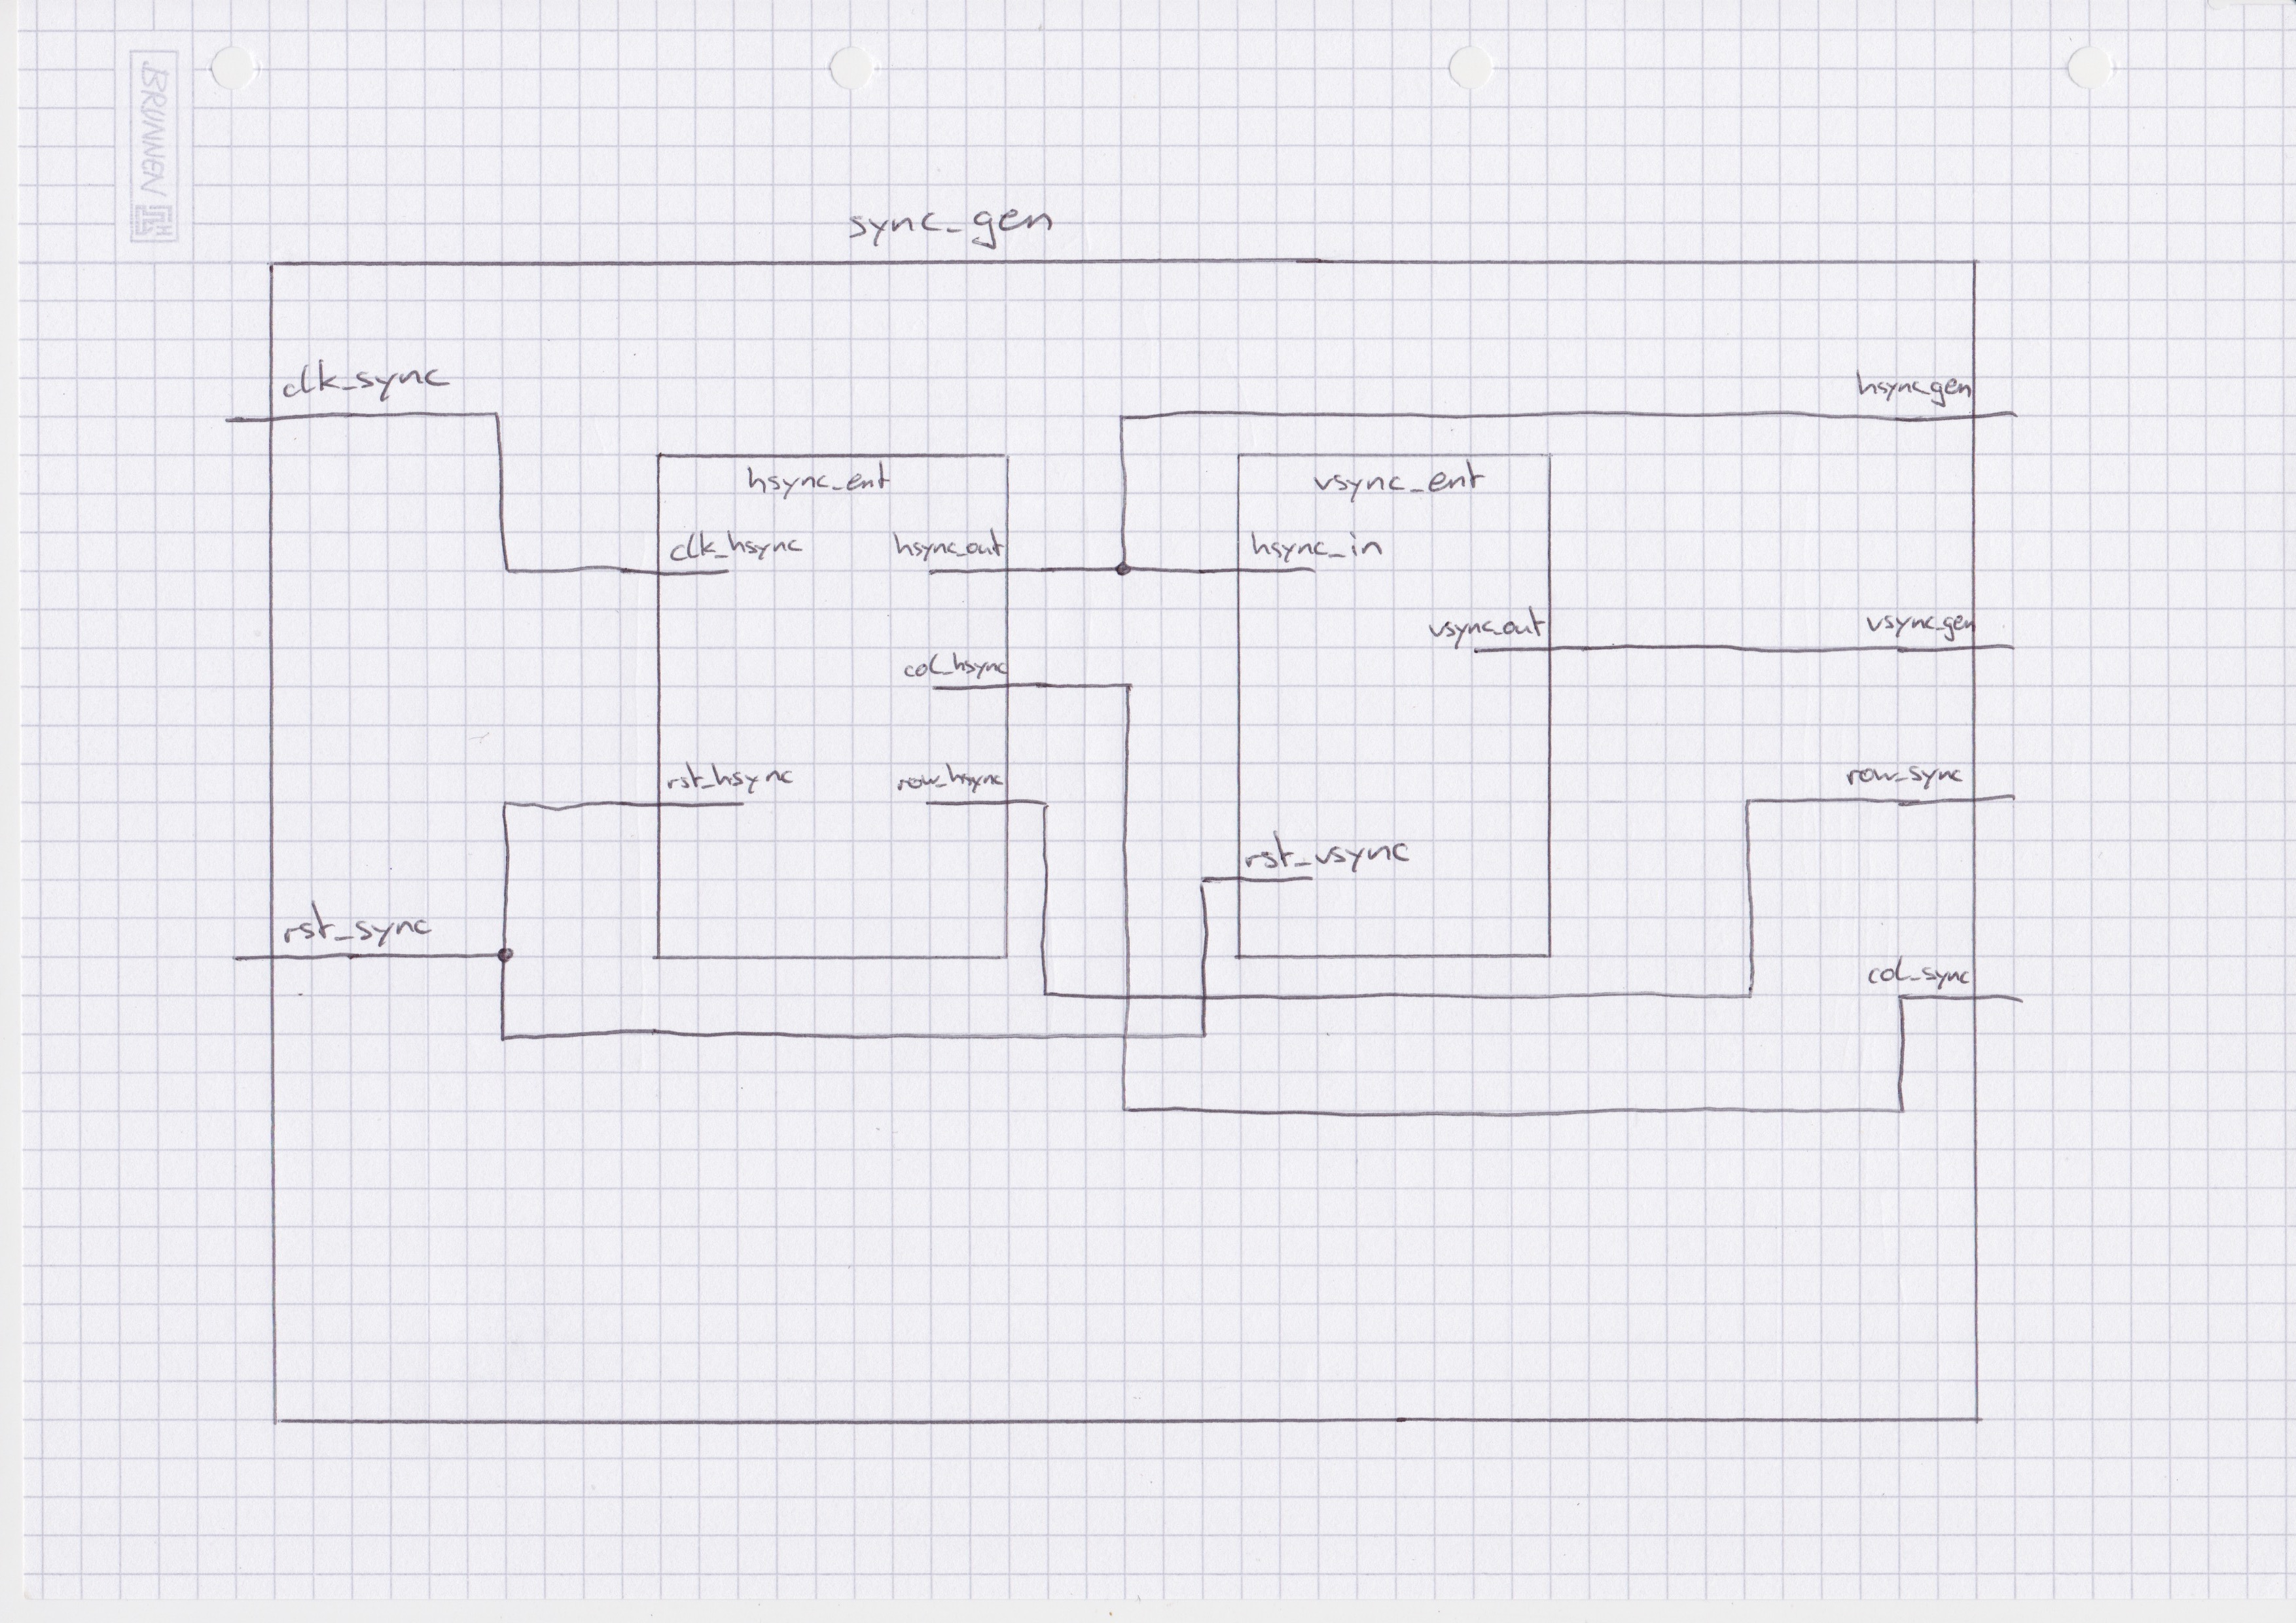
\includegraphics[scale=0.1]{./bilder/Sync_gen.jpeg}
				\caption{Blockdiagramm sync\_gen\_ent}
			\end{figure}
		
	\part{Probleme}
		\section{Allgemein}
			\begin{itemize}
				\item In einer Version unseres Designs hatten wir ein \enquote{congested design}, was sich darin äußerte, dass Place \& Route mehrere Stunden dauerte und nicht zu einem Ende kam. Wir lösten dieses Problem, indem wir unnötige Ports (und somit Leitungen) aus unserem Design löschten. Dies kam vor allen Dingen bei der player\_ent zum Tragen, da wir hier zu Beginn jedem Player alle 15 Rows übergaben, wobei für die Kollision bei der Bewegung nur maximal drei Rows benötigt werden. Durch die Reduktion der Ports auf diese drei Rows wurde Place \& Route deutlich beschleunigt und das Design konnte implementiert werden.
				\item Hin und wieder (nicht reproduzierbar) passieren gefühlt zufällige, unerwartete Dinge. Zum Beispiel werden eine oder mehrere Rows komplett leer oder es tauchen einzelne schwarze Blöcke auf (für schwarze Blöcke existiert in unserem Code überhaupt keine Logik).
			\end{itemize}

		\section{game\_mechanic\_ent}

			\subsection{game\_state\_ent}
				\begin{itemize}
					\item Das größte Problem war die korrekte Darstellung der Explosionen. Sobald eine Bombe explodiert ist, wurde in der mittleren Zeile nur eine Explosion dargestellt, obwohl es eigentlich drei Felder mit Explosionen sein sollten. Um die Zeilen zu ändern hatten wir eine eigene Funktion, die die Änderungen vornimmt. Dort wurde immer eine lokale Kopie der entsprechenden Zeile gespeichert, dann die Änderung vorgenommen und anschließend die alte Zeile durch die neue überschrieben. Das Problem war, dass wir diese Funktion für alle fünf Blöcke, die bei einer Explosion geändert werden müssen, nacheinander aufgerufen haben und dies somit parallel ausgeführt wird. Bei den Explosionen über und unter der Bombe führte dies zu keinem Problem, allerdings bei denen rechts und links der Bombe. Die Funktion wurde hier also parallel ausgeführt und immer wurde eine lokale Kopie der Zeile gespeichert und später zurückgeschrieben. Sobald die letzte Änderung in einer Zeile vorgenommen wurde, wurden alle Änderungen die durch andere Funktionsaufrufe auf diese Zeile ausgeführt wurden, überschrieben und somit wurde immer nur eine anstatt drei Explosionen dargestellt. Dieses Problem haben wir behoben, indem wir die Funktion nicht fünf Mal aufgerufen haben, sondern nur einmal und dieser eine Aufruf sorgt direkt für alle fünf Änderungen.
				\end{itemize}

			\subsection{player\_ent}

				\subsubsection{movement\_ent}
					\begin{itemize}
						\item Lange Zeit hatten wir ein Problem damit, dass die Spielfiguren in Blöcke hineinglitchen konnten, falls sie sich auf zwei Kacheln gleichzeitig befanden und in Richtung des Blockes bewegten. Der Fehler ergab sich wie folgt: 
						Um die Position des rechtesten Pixels eines Spielers herauszufinden (wird für die Kollisionserkennung benötigt), haben wir eine Variable x\_right, welche wir nach jeder Bewegung in x-Richtung aktualisieren. Diese ergibt sich im Wesentlichen durch Addieren der Spielergröße (Generic) auf die aktuelle x-Position des Spielers. 
						Unser Fehler bestand nun darin, dass wir für die Neuberechnung von x\_right nach jeder Bewegung in x-Richtung X\_INIT (Generic, das die initiale x-Position des Spielers enthält) statt x\_int (Variable, die die aktuelle x-Position des Spielers enthält) verwendeten.
						\item Zu Beginn bekam movement\_ent alle 15 Rows des Spielfeldes, was wir gegen Ende noch änderten. Nun werden nur die zur Kollision benötigten Rows übergeben. 
						Dies führte zu Problemen, da wir nun die zu prüfenden Rows anders auswählen mussten. Ein Fehler in unserer diesbezüglichen Logik führte dazu, dass die Bewegung in bestimmte Richtungen nicht mehr möglich war, da wir nun stets alle in Frage kommenden Kacheln überprüften und nicht nur die benötigten. Dieses Problem ließ sich allerdings leicht lösen, indem wir im Falle, dass der Spieler sich auf exakt einer Kachel befindet wir nur eine Kachel zur Kollision überprüfen.
						\item Am Ende des Praktikums haben wir mit der Bewegung der Spieler noch zwei größere Probleme:
						\begin{itemize}
							\item In der rechten Hälfte der Arena (ab der neunten Spalte) funktioniert die Bewegung nicht wie von uns erwartet. Von dort ist eine Bewegung nach links nicht mehr möglich und auch die Kollision mit Blöcken funktioniert nicht mehr ordnungsgemäß. Woran das liegt, haben wir nicht mehr herausgefunden, da das Verhalten in der Simulation so nicht vorkommt.
							\item %TODO diagonal glitchen?
						\end{itemize}
					\end{itemize}
					
		\section{graphics\_ent}

			\subsection{pixel\_gen\_ent}
				\begin{itemize}
					\item Ein Problem war hier die falsche Berechnung des Offsets für den zweiten Spieler. Hier haben wir vergessen die 160 Pixel des schwarzen Randes zu subtrahieren. Dieser Offset wird für den Zugriff auf den Sprite verwendet.
					\item Ein weiteres Problem war die Art, wie wir das Speilfeld zeichnen. Ursprünglich haben wir entweder das Spielfeld oder einen Spieler gezeichnet. Als wir jedoch Sprites benutzen wollten, mussten wir dies ändern, um die transparenten Bereiche in dem Sprite des Spielers auch tatsächlich transparent zeichnen zu können. Dafür mussten wir weitere Ausgänge für die Spieler hinzufügen, um Informationen über den Sprite unterhalb des Spielers, sowie über den Sprite des Spielers weitergeben zu können.
				\end{itemize}
			
			\subsection{Sprites}
				\begin{itemize}
					\item Bei der ersten Implementierung geschah der Zugriff auf die ROMs taktsynchron. Dies führte zu einer Ausgabe, die verschmiert und deutlich dunkler als erwartet war. Erklären ist dies damit, dass durch die Taktsynchronität der RGB-Wert eines Pixels aus der Top-Level-Entity zwei Takte zu spät ausgegeben wurde (SpriteROM und PlayerROM verzögern Ausgabe jeweils um einen Takt). Somit wurden am Ende jeder Zeile des Bildes jeweils zwei Takte zu lang RGB-Werte gesetzt, was bei der VGA-Signalgenerierung allerdings nicht erlaubt ist.
					Gelöst wurde das Problem dadurch, dass SpriteROM und PlayerROM nun asynchron arbeiten.
				\end{itemize}
	
		
		\section{sync\_gen\_ent}
			Ein Problem, das schon bei der Lösung des Übungsblatts aufgetaucht ist, hat sich auch durch das Projekt gezogen.
			Die VGA-Ausgabe funktioniert nicht an allen Monitoren ordnungsgemäß (es tritt ein Flackern auf). An unserem Test-Monitor hat die VGA-Ausgabe nach einigen Einstellungen jedoch funktioniert.
\end{document}